\documentclass{article}

\usepackage[margin=0.5in]{geometry}
\usepackage[inter-unit-product=\cdot,per-mode=symbol]{siunitx}
\usepackage{float}
\usepackage{amsmath}
\usepackage{commath}
\usepackage{vwcol}
\usepackage{multicol}
\usepackage{graphicx}
\usepackage{caption, copyrightbox}
\usepackage{url}

\captionsetup{justification=centering, labelfont=sc, labelsep=endash}

\title{Astronautics Cheat Sheet}

\newcommand{\myvarmukm}{\mu &= \text{Gravitational parameter \si{\kilo\meter\cubed\per\sec\squared}} \approx 3.986 \times 10^5 \si{\kilo\meter\cubed\per\second\squared} \text{ for Earth}} 

\newcommand{\myvarv}{V &= \text{spacecraft's velocity (\si{\kilo\meter\per\sec})}}

\newcommand{\myvarepsilon}{\varepsilon &= \text{spacecraft's specific mechanical energy (\si{\kilo\meter\squared\per\second\squared)}}}

\newcommand{\myvara}{a &= \text{semimajor axis (\si{\kilo\meter})}}

\begin{document}
\maketitle

\section{Math review}
\subsection{Trigonometry}
	\begin{figure}[H]
		\centering
		\includegraphics[width=0.4\linewidth]{img/trigo_triangle}
		\label{fig:trigo_triangle}
	\end{figure}

\subsubsection*{SOH-CAH-TOA}

\begin{itemize}
	\item $\sin$ $\theta$ = Opposite / Hypotenuse
	\item $\cos$ $\theta$ = Adjacent / Hypotenuse
	\item $\tan$ $\theta$ = Opposite / Adjacent
\end{itemize}

\subsubsection*{Spherical Trigonometry}
TODO

\subsection{Vector math}
\subsubsection*{Vector components}
$\vec{A} = A_I\hat{I} + A_J\hat{J} + A_K\hat{K}$

\subsubsection*{Magnitude of vector}
$\lVert\vec{A}\rVert = A = \sqrt{A_I^2 + A_J^2 + A_K^2}$

\subsubsection*{Vector addition}
$\vec{A} + \vec{B} = (A_I + B_I)\hat{I} + (A_J + B_J)\hat{J} + (A_K + B_K)\hat{K}$

\subsubsection*{Scalar or dot product}

\begin{multicols}{3}
	\begin{figure}[H]
		\centering
		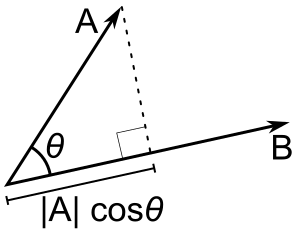
\includegraphics[width=0.6\linewidth]{img/dot_product}
		\caption{Dot product}
		\label{fig:dot_product}
	\end{figure}

	\columnbreak
	\begin{equation*}
	\boxed{\vec{A}\cdot\vec{B} = AB\cos\theta}
	\end{equation*}

	\begin{equation*}
	\boxed{\vec{A}\cdot\vec{B} = (A_IB_I) + (A_JB_J) + (A_KB_K)}
	\end{equation*}

	\vfill\null
	\columnbreak

	\begin{equation*}
	\boxed{\theta = \cos^-1 \dfrac{\vec{A}\cdot\vec{B}}{AB}}
	\end{equation*}
\end{multicols}

\subsubsection*{Vector or cross product}
	\begin{multicols}{2}
	\begin{figure}[H]
		\centering
		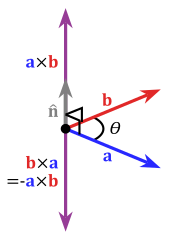
\includegraphics[width=0.5\linewidth]{img/cross_product_vector}
		\caption{Cross product}
		\label{fig:right_hand_rule}
	\end{figure}
	\vfill\null
	\columnbreak
	\begin{figure}[H]
		\centering
		\copyrightbox[r]{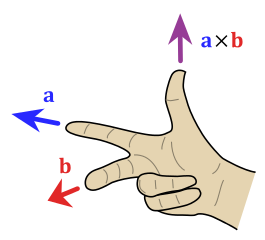
\includegraphics[width=0.7\linewidth]{img/right_hand_rule_cross_product}}{\textcopyright Acdx, CC BY-SA 3.0 \url{http://creativecommons.org/licenses/by-sa/3.0/>}, via Wikimedia Commons \url{https://commons.wikimedia.org/wiki/File:Right_hand_rule_cross_product.svg>}}
		\caption{Right hand rule}
		\label{fig:right_hand_rule}
	\end{figure}

	\end{multicols}

	\begin{equation*}
	\boxed{\vec{A} \times \vec{B} = [(A_J)(B_K)-(B_J)(A_K)]\hat{I} - [(A_I)(B_K) - (B_I)(A_K)]\hat{J} + [(A_I)(B_J)-(B_I)(A_J)]}
	\end{equation*}
	
	\begin{equation*}
	\boxed{\lVert\vec{A} \times \vec{B}\rVert = AB\sin\theta}
	\end{equation*}

\section{Constants}
\begin{center}
	\begin{tabular}{|c | c |  c | c |} 
		\hline
		Symbol & Name & value & unit \\ [0.5ex] 
		\hline\hline
		& Earth radius & 6378.14 & km \\ 
		\hline
		$\mu$ & Gravitational parameter & $3.986 \times 10^{14}$ & \si{\meter\cubed\per\second\squared} \\ 
		\hline
	\end{tabular}
\end{center}

\section{Newton's laws of motion}
\subsection{Newton's first law of motion}
\begin{multicols}{2}
A body continues in its state of rest, or of uniform motion in a straight line, unless compelled to change that state by forces impressed upon it.
\vfill\null
\columnbreak
\begin{equation*}
	\boxed{\vec{p} = m\vec{V}}
\end{equation*}

\begin{align*}
\vec{p} &= \text{linear momentum vector (\si{\kilo\gram\meter\per\second})}\\
m &= \text{mass (\si{\kilo\gram})}\\
\vec{V} &= \text{velocity vector (\si{\meter\per\second})}\\
\end{align*}

\end{multicols}

\begin{multicols}{2}
\begin{equation*}
\boxed{\vec{H} = I\vec{\Omega}}
\end{equation*}

\begin{align*}
\vec{H} &= \text{angular momentum vector (\si{\kilo\gram\meter\squared\per\second})}\\
I &= \text{moment of inertia (\si{\kilo\gram\meter\squared})}\\
\vec{\Omega} &= \text{angular velocity vector (\si{\radian\per\second})}\\
\end{align*}

\vfill\null
\columnbreak

\begin{equation*}
\boxed{\vec{H} = \vec{R} \times m\vec{V}}
\end{equation*}

\begin{align*}
\vec{H} &= \text{angular momentum vector (\si{\kilo\gram\meter\squared\per\second})}\\
\vec{R} &= \text{position (\si{\meter})}\\
m &= \text{mass (\si{\kilo\gram})}\\
\vec{V} &= \text{velocity vector (\si{\meter\per\second})}\\
\end{align*}
\vfill\null
\end{multicols}

\subsection{Newton's second law of motion}
\begin{multicols}{2}
	The time rate of change of an object's momentum equals the applied force.
	\vfill\null
	\columnbreak
	\begin{equation*}
	\boxed{\vec{F} = m\vec{a}}
	\end{equation*}

	\begin{align*}
	\vec{F} &= \text{force vector (\si{\kilo\gram\meter\per\second\squared = \newton})}\\
	m &= \text{mass (\si{\kilo\gram})}\\
	\vec{a} &= \text{acceleration  (\si{\meter\per\second\squared})}\\
	\end{align*}
\end{multicols}

\subsection{Newton's third law of motion}
When body A exerts a force on body B, body B will exert an equal, but opposite, force on body A

\section{Newton's laws of universal gravitation}
\begin{multicols}{3}

	\begin{equation*}
	\boxed{F_{g} = \dfrac{Gm_{1}m_{2}}{R^{2}}}
	\end{equation*}
	\vfill\null
	\columnbreak
	\begin{align*}
	F_{g} &= \text{force due to gravity (\si{\newton})}\\
	G &= \text{universal gravitational constant} \approx
	  6.674 \times 10^{-11}\,\si{\newton \meter\squared\per\kilo\gram\squared}\\
	m_{1}, m_{2} &= \text{masses of two bodies  (\si{\kilo\gram})}\\
	R &= \text{distance between the two bodies  (\si{\meter})}\\
	\end{align*}
\end{multicols}
\begin{multicols}{3}
	\begin{equation*}
	\boxed{a_{g} = \dfrac{\mu_{Earth}}{R^{2}}}
	\end{equation*}
	\vfill\null
	\columnbreak
	\begin{align*}
	a_{g} &= \text{acceleration due to gravity (\si{\meter\per\second\squared})}\\
	\mu_{Earth} &\equiv G\,m_{Earth} \approx 3.986 \times 10^{14} \, \si{\meter\cubed\per\second\squared}\\
	R &= \text{distance between the two bodies  (\si{\meter})}\\
	\end{align*}

	\vfill\null
\end{multicols}

\section{Laws of conservation}
\subsection{Conservation of momentum}
In the absence of outside forces, linear and angular momentum are conserved.

\subsection{Energy}
\begin{multicols}{3}
	\begin{equation*}
	\boxed{E = KE + PE}
	\end{equation*}

	\begin{align*}
	E &= \text{total mechanical energy (\si{\kilo\gram\,\meter\squared\per\second\squared)}}\\
	KE &= \text{kinetic energy (\si{\kilo\gram\,\meter\squared\per\second\squared)}}\\
	PE &= \text{potential energy (\si{\kilo\gram\,\meter\squared\per\second\squared)}}\\
	\end{align*}

	\vfill\null
	\columnbreak

	\begin{equation*}
	\boxed{PE = m\,a_{g}h}
	\end{equation*}

	\begin{align*}
	m &= \text{mass (\si{\kilo\gram})}\\
	a_{g} &= \text{acceleration due to gravity (\si{\meter\per\second\squared})}\\
	h &= \text{height above ref. point (\si{\meter})}\\
	\end{align*}
	\vfill\null
	\columnbreak

	\begin{equation*}
	\boxed{PE = -\dfrac{m\mu}{R}}
	\end{equation*}

	\begin{align*}
	m &= \text{spacecraft's mass (\si{\kilo\gram})}\\
	\mu &= \text{gravitational parameter (\si{\kilo\meter\cubed\per\second\squared})}\\
	R &= \text{distance from Earth's center (\si{\kilo\meter})}\\
	\end{align*}
	\vfill\null
\end{multicols}

\begin{multicols}{2}
	\begin{equation*}
	\boxed{KE = \dfrac{1}{2} m V^{2}}
	\end{equation*}

	\begin{align*}
	KE &= \text{kinetic energy (\si{\kilo\gram\,\meter\squared\per\second\squared)}}\\
	m &= \text{mass (\si{\kilo\gram})}\\
	V &= \text{velocity (\si{\kilo\meter\per\second}})\\
	\end{align*}

	\vfill\null
	\columnbreak

	\begin{equation*}
	\boxed{E = \dfrac{1}{2} m V^{2} - \dfrac{m\mu}{R}}
	\end{equation*}

	\begin{align*}
	E &= \text{total mech. energy (\si{\kilo\gram\,\meter\squared\per\second\squared)}}\\
	m &= \text{mass (\si{\kilo\gram})}\\
	V &= \text{velocity (\si{\kilo\meter\per\second}})\\
	\mu &= \text{gravitational parameter (\si{\kilo\meter\cubed\per\second\squared})}\\
	R &= \text{position (\si{\kilo\meter})}\\
	\end{align*}
	\vfill\null
\end{multicols}

\section{The restricted two-body problem}
\subsection{Coordinate systems}

\begin{figure*}[!h]
	\centering
	\copyrightbox[r]{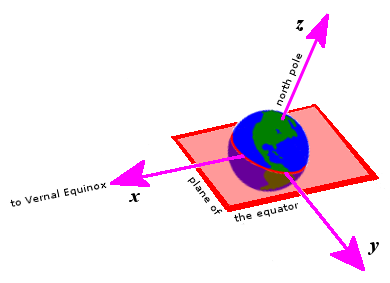
\includegraphics[width=0.7\linewidth]{img/Ra_and_dec_rectangular}}{\textcopyright By Tfr000 (talk) 19:24, 23 April 2012 (UTC) - Own work, CC BY-SA 3.0, https://commons.wikimedia.org/w/index.php?curid=19193590}
	\caption{Geocentric equatorial coordinates. The origin is the centre of the Earth. The fundamental plane is the plane of the Earth's equator. The primary direction (the x axis) is the vernal equinox. A right-handed convention specifies a y axis 90° to the east in the fundamental plane; the z axis is the north polar axis. The reference frame does not rotate with the Earth, rather, the Earth rotates around the z axis.}
	\label{fig:coordinate_system}
\end{figure*}

A coordinate system (figure \ref{fig:coordinate_system}) is:
\begin{itemize}
	\item \textbf{an origin}
	\item \textbf{a fundamental plane}, containing two axes, and the perpendicular to it
	\item \textbf{a principal direction} within the plane
	\item \textbf{the third axis} using the right-hand rule
\end{itemize}

\subsection{Equation of motion}
\begin{equation*}
\boxed{\ddot{\vec{R}} + \dfrac{\mu}{R^{2}} \dfrac{\vec{R}}{R} = 0}
\end{equation*}

\begin{align*}
\ddot{\vec{R}} &= \text{spacecraft's acceleration (\si{\kilo\meter\per\second\squared})}\\
\mu &= \text{gravitational parameter (\si{\kilo\meter\cubed\per\second\squared})}\\
\vec{R} &= \text{spacecraft's position vector (\si{\kilo\meter})}\\
R &= \text{magnitude of the spacecraft's position vector (\si{\kilo\meter})}\\
\end{align*}

\subsection{Orbital geometry}

\begin{minipage}{0.6\textwidth}
	\begin{figure}[H]
		\centering
		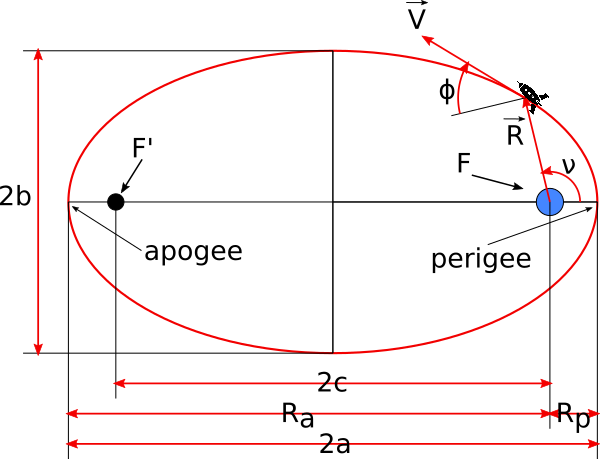
\includegraphics[width=0.9\linewidth]{img/ellipse}
		\caption{Geometry of an elliptical orbit}
		\label{fig:coordinate_system}
	\end{figure}
\end{minipage} \hfill
\begin{minipage}{0.35\textwidth}
	\begin{align*}
	\vec{R} &= \text{spacecraft's position vector}\\
	\vec{V} &= \text{spacecraft's velocity vector}\\
	F and F' &= \text{primary and vacant foci}\\
	R_{p} &= \text{radius of perigee}\\
	R_{a} &= \text{radius of apogee}\\
	2a &= \text{major axis}\\
	2b &= \text{minor axis}\\
	2c &= \text{distance between the foci}\\
	a &= \text{semimajor axis}\\
	b &= \text{semiminor axis}\\
	\nu &= \text{true anomaly}\\
	\phi &= \text{flight-path angle}\\
	\end{align*}
\end{minipage}

\begin{samepage}
\begin{multicols}{2}
	\begin{equation*}
	\boxed{e = \dfrac{2c}{2a} = \dfrac{R_{a} - R_{p}}{R_{a} + R_{p}}}
	\end{equation*}

	\begin{align*}
	e = eccentricity\\
	\end{align*}
	\vfill\null
	\columnbreak

	\begin{equation*}
	\boxed{R = \dfrac{a ( 1 - e^{2})}{1 + e cos \nu}}
	\end{equation*}

	\begin{align*}
	R &= \text{magnitude of the spacecraft's position vector (km)}\\
	a &= \text{semi-major axis (km)}\\
	e &= \text{eccentricity (unitless)}\\
	\nu &= \text{true anomaly (deg or rad)}\\
	\end{align*}
\end{multicols}
\end{samepage}

\begin{center}
	\begin{tabular}{|c | c | c | c|} 
		\hline
		Conic section & a = semimajor axis & c = one half the distance between foci & e = eccentricity \\ [0.5ex] 
		\hline\hline
		circle & a $>$ 0 & c = 0 & e = 0 \\ 
		\hline
		ellipse & a $>$ 0 & 0 $<$ c $<$ a & 0 $<$ e $<$ 1 \\
		\hline
		parabola & a = $\infty$ & c = $\infty$ & e = 1 \\
		\hline
		hyperbola & a $<$ 0 & \abs{a} $<$ \abs{c} $>$ 0 & e $>$ 1 \\
		\hline
	\end{tabular}
\end{center}

\section{Constants of orbital motion}
\subsection{Specific mechanical energy}

\begin{multicols}{3}
	\begin{equation*}
	\boxed{\varepsilon \equiv \dfrac{E}{m} = \dfrac{V^2}{2} - \dfrac{\mu}{R}}
	\end{equation*}

	\begin{equation*}
	\boxed{V = \sqrt{2(\dfrac{\mu}{R} + \varepsilon)}}
	\end{equation*}

	\vfill\null
	\columnbreak

	\begin{align*}
	\myvarepsilon\\
	\myvarv\\
	\myvarmukm \\
	R &= \text{spacecraft's distance from Earth's center (\si{\kilo\meter})}\\
	\end{align*}
\end{multicols}

\begin{multicols}{3}
	\begin{equation*}
	\boxed{\varepsilon = - \dfrac{\mu}{2a}}
	\end{equation*}

	\vfill\null
	\columnbreak

	\begin{align*}
	\myvarepsilon\\
	\myvarmukm \\
	\myvara\\
	\end{align*}
\end{multicols}

\begin{multicols}{3}
	\begin{equation*}
	\boxed{P = 2\pi\sqrt{\dfrac{a^3}{\mu}}}
	\end{equation*}

	\vfill\null
	\columnbreak

	\begin{align*}
	P &= \text{period (seconds)}\\
	\pi &= \text{3.14159... (unitless)}\\
	\myvara\\
	\myvarmukm \\
	\end{align*}
\end{multicols}

\subsection{Specific angular momentum}
\begin{multicols}{3}
	\begin{equation*}
	\boxed{\vec{h} \equiv \dfrac{\vec{H}}{m} = \vec{R} \times \vec{V}}
	\end{equation*}

	\vfill\null
	\columnbreak

	\begin{align*}
	\vec{h} &= \text{spacecraft's specific angular momentum (\si{\kilo\meter\squared\per\second})}\\
	\vec{R} &= \text{spacecraft's position vector (\si{\kilo\meter})}\\
	\vec{V} &= \text{spacecraft's velocity vector (\si{\kilo\meter\per\second})}\\
	\end{align*}
\end{multicols}

\section{Describing orbits}
\subsection{Orbital elements}
\begin{itemize}
	\item Size: semimajor axis, a
	\item Shape: eccentricity, e
	\item Tilt: inclination, i
	\item Angle from vernal equinox to ascending node: right ascension (or longitude) of ascending node, $\Omega$
	\item Angle from AN to Pe: argument of perigee, $\omega$
	\item Angle from Pe to spacecraft: true anomaly, $\nu$
\end{itemize}

\begin{figure*}[!h]
	\centering
	\copyrightbox[r]{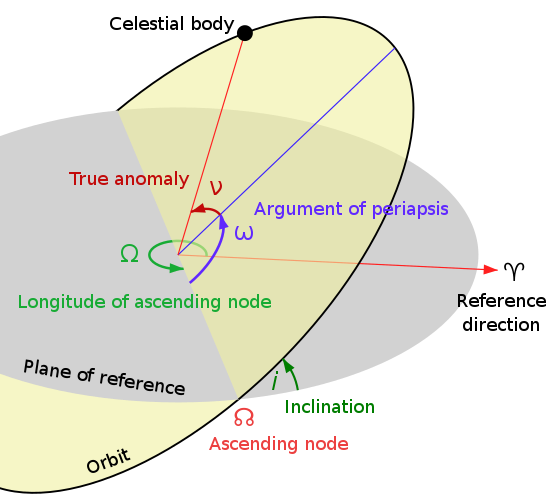
\includegraphics[width=0.6\linewidth]{img/orbit_elements}}{\textcopyright Lasunncty at the English Wikipedia \url{https://upload.wikimedia.org/wikipedia/commons/e/eb/Orbit1.svg}, CC BY-SA 3.0 \url{http://creativecommons.org/licenses/by-sa/3.0/}, via Wikimedia Commons}
	\caption{Orbital elements}
	\label{fig:coordinate_system}
\end{figure*}

\subsection{Computing orbital elements} \label{computing_orbital_elements}
Knowing $\vec{R}$ and $\vec{V}$ from ground tracking, we can compute orbital elements:

\begin{multicols}{3}
\begin{equation*}
\boxed{\varepsilon = \dfrac{V^2}{2} - \dfrac{\mu}{R}}
\end{equation*}

\begin{equation*}
\boxed{a = - \dfrac{\mu}{2 \varepsilon}}
\end{equation*}

\vfill\null
\columnbreak

\begin{align*}
\myvarepsilon\\
\myvarv\\
\myvarmukm \\
R &= \text{spacecraft's distance from Earth's center (\si{\kilo\meter})}\\
\end{align*}
\end{multicols}

\begin{multicols}{3}
	\begin{equation*}
	\boxed{\vec{e} = \dfrac{1}{\mu}\left[\left(V^2 - \dfrac{\mu}{R}\right)\vec{R} - (\vec{R}\cdot\vec{V})\vec{V}\right]}
	\end{equation*}

	\vfill\null
	\columnbreak

	\begin{align*}
	\vec{e} &= \text{eccentricity vetor (unitless, points at Pe)}\\
	\myvarmukm \\
	V &= \text{magnitude of $\vec{V}$ (\si{\kilo\meter\per\second})}\\
	R &= \text{magnitude of $\vec{R}$ (\si{\kilo\meter})}\\
	\vec{R} &= \text{position vector (\si{\kilo\meter})}\\
	\vec{V} &= \text{velocity vector (\si{\kilo\meter\per\second})}\\
	\end{align*}
\end{multicols}

\begin{multicols}{3}
	\begin{equation*}
	\boxed{i = \cos^{-1}\left(\dfrac{\hat{K} \cdot \vec{h}}{K h}\right)}
	\end{equation*}

	\begin{equation*}
	0 \leq i \leq 180^\circ
	\end{equation*}
	\vfill\null
	\columnbreak

	\begin{align*}
	i &= \text{inclination (\si{\deg \text{or } \radian})}\\
	\hat{K} &= \text{unit vector through the North Pole}\\
	\vec{h} &= \text{specific angular momentum vector (\si{\kilo\meter\squared\per\second})}\\
	K &= \text{magnitude of $\hat{K}$ = 1}\\
	h &= \text{magnitude of $\vec{h}$ (\si{\kilo\meter\squared\per\second})}\\
	\end{align*}
\end{multicols}

\begin{multicols}{3}
	\begin{equation*}
	\boxed{\vec{n} = \hat{K} \times \vec{h}}
	\end{equation*}
	\vfill\null
	\columnbreak

	\begin{align*}
	\vec{n} &= \text{ascending node vector (\si{\kilo\meter\squared\per\second}, points at the ascending node)}\\
	\hat{K} &= \text{unit vector through the North Pole}\\
	\vec{h} &= \text{specific angular momentum vector (\si{\kilo\meter\squared\per\second})}\\
	\end{align*}
\end{multicols}

\begin{multicols}{3}
	\begin{equation*}
	\boxed{\Omega = \cos^{-1}\left(\dfrac{\hat{I} \cdot \vec{n}}{In}\right)}
	\end{equation*}

	\begin{equation*}
	 \text{if } n_j \geq 0 \text{ then } 0 \leq \Omega \leq 180^\circ
	\end{equation*}
	\begin{equation*}
	\text{if } n_j < 0 \text{ then } 180^\circ < \Omega < 360^\circ
 	\end{equation*}

	\vfill\null
	\columnbreak

	\begin{align*}
	\Omega &= \text{right ascension of the ascending node (\si{\deg \text{or } \radian})}\\
	\hat{I} &= \text{unit vector in the principal direction}\\
	\vec{n} &= \text{ascending node vector (\si{\kilo\meter\squared\per\second}, points at the ascending node)}\\
	I &= \text{magnitude of $\hat{I}$ = 1}\\
	n &= \text{magnitude of $\vec{n}$ (\si{\kilo\meter\squared\per\second})}\\
	\end{align*}
\end{multicols}

\begin{multicols}{3}
	\begin{equation*}
	\boxed{\omega = \cos^{-1} \left(\dfrac{\vec{n}\cdot\vec{e}}{ne}\right)}
	\end{equation*}
	
	\begin{equation*}
	\text{if } e_K \geq 0 \text{ then } 0 \leq \omega \leq 180^\circ
	\end{equation*}
	\begin{equation*}
	\text{if } e_K < 0 \text{ then } 180^\circ < \omega < 360^\circ
	\end{equation*}

	\vfill\null
	\columnbreak

	\begin{align*}
	\omega &= \text{argument of perigee (\si{\deg \text{or } \radian})}\\
	\vec{n} &= \text{ascending node vector (\si{\kilo\meter\squared\per\second}, points at the ascending node)}\\
	\vec{e} &= \text{eccentricity vector (unitless, points at perigee)}\\
	n &= \text{magnitude of $\vec{n}$ (\si{\kilo\meter\squared\per\second})}\\
	e &= \text{magnitude of $\vec{e}$ (unitless)}\\
	\end{align*}
\end{multicols}

\begin{multicols}{3}
	\begin{equation*}
	\boxed{\nu = \cos^{-1} \left(\dfrac{\vec{e}\cdot\vec{R}}{eR}\right)}
	\end{equation*}
	
	\begin{equation*}
	\text{if } \vec{R}\cdot\vec{V} \geq 0 \text{ then } 0 \leq \nu \leq 180^\circ
	\end{equation*}
	\begin{equation*}
	\text{if } \vec{R}\cdot\vec{V} < 0 \text{ then } 180^\circ < \nu < 360^\circ
	\end{equation*}

	\vfill\null
	\columnbreak

	\begin{align*}
	\nu &= \text{true anomaly (\si{\deg \text{or } \radian})}\\
	\vec{e} &= \text{eccentricity vector (unitless, points at perigee)}\\
	\vec{R} &= \text{position vector (\si{\kilo\meter}}\\
	e &= \text{magnitude of $\vec{e}$ (unitless)}\\
	R &= \text{magnitude of $\vec{R}$ (\si{\kilo\meter})}\\
	\end{align*}
\end{multicols}

\subsection{Ground tracks}
Nodal displacement: displacement of orbit to the west between each revolution

\begin{equation*}
\boxed{\Delta N = 360^\circ - \text{longitude between successive ascending nodes}}
\end{equation*}

\begin{equation*}
\boxed{\text{Period (hours)} = \dfrac{\Delta N}{15^\circ / hr}}
\text{ for direct orbits only} (0 < i < 90^\circ)
\end{equation*}

\begin{multicols}{3}
	\begin{equation*}
	\boxed{a = \sqrt[3]{\mu (P / 2\pi)}}
	\end{equation*}
	
	\vfill\null
	\columnbreak
	
	\begin{align*}
	a &= \text{semimajor axis (\si{\kilo\meter)}}\\
	\myvarmukm\\
	P &= \text{period (\si{\second})}\\
	\pi &= 3.14159... \text{(unitless)}\\
	\end{align*}
\end{multicols}

inclination = highest latitude

\begin{itemize}
	\item For a direct orbit ($0 < i < 90^\circ$), inclination = highest north or south latitude.
	\item For a retrograde orbit ($90^\circ < i < 180^\circ$), inclination = 180 - max latitude
\end{itemize}

\section{Maneuvers}
\subsection{Hohmann Transfers}

\begin{figure*}[!h]
	\centering
	\copyrightbox[r]{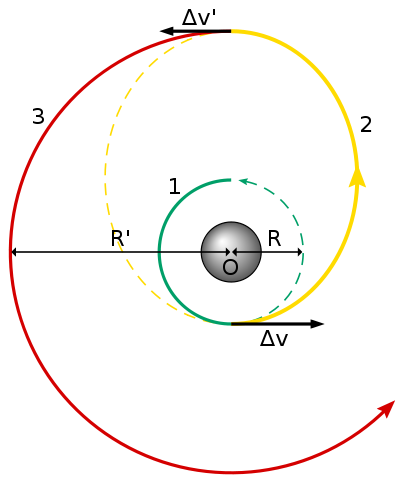
\includegraphics[width=0.5\linewidth]{img/hohmann_transfer}}{\textcopyright Leafnode \url{https://commons.wikimedia.org/wiki/File:Hohmann_transfer_orbit.svg} CC BY-SA 2.5 \url{https://creativecommons.org/licenses/by-sa/2.5}, via Wikimedia Commons}
	\caption{Transfer orbit}
	\label{fig:coordinate_system}
\end{figure*}

Specific mechanical energy of each orbit:

\begin{itemize}
	\item $\varepsilon_{\text{orbit 1}} = -\dfrac{\mu}{2a_{\text{orbit 1}}}$
	\item $\varepsilon_{\text{orbit 2}} = -\dfrac{\mu}{2a_{\text{orbit 2}}}$
	\item $\varepsilon_{transfer} = -\dfrac{\mu}{2a_{transfer}}$ with $2a_{transfer} = R + R'$
\end{itemize}

Velocity at each maneuver point using specific mechanical energy equation from section \ref{computing_orbital_elements}:

\begin{multicols}{2}
	\begin{itemize}
		\item $V_{\text{orbit 1}} = \sqrt{2\left(\dfrac{\mu}{R} + \varepsilon_{\text{orbit 1}}\right)}$
		\item $V_{\text{orbit 2}} = \sqrt{2\left(\dfrac{\mu}{R'} + \varepsilon_{\text{orbit 2}}\right)}$
		\item $V_{\text{transfer at orbit 1}} = \sqrt{2\left(\dfrac{\mu}{R} + \varepsilon_{transfer}\right)}$
		\item $V_{\text{transfer at orbit 2}} = \sqrt{2\left(\dfrac{\mu}{R'} + \varepsilon_{transfer}\right)}$
	\end{itemize}
	\vfill\null
	\columnbreak
	\begin{itemize}
		\item $\Delta V_1 = |V_{\text{transfer at orbit 1}} - V_{\text{orbit 1}}|$
		\item $\Delta V_2 = |V_{\text{orbit 2}} - V_{\text{transfer at orbit 2}}|$
		\item $\Delta V_{total} = \Delta V_1 + \Delta V_2$
	\end{itemize}
\end{multicols}

Time of flight = half period

\begin{multicols}{3}
	\begin{equation*}
	\boxed{TOF = \dfrac{P}{2} = \pi \sqrt{\dfrac{a_{transfer}^3}{\mu}}}
	\end{equation*}
	
	\vfill\null
	\columnbreak
	
	\begin{align*}
	TOF &= \text{spacecraft's time of flight}\\
	P &= \text{orbital period (\si{\second})}\\
	a &= \text{semimajor axis of transfer orbit (\si{\kilo\meter)}}\\
	\myvarmukm\\
	\end{align*}
\end{multicols}

\end{document}
